% Chapter Template

\chapter{Introducción específica} % Main chapter title

\label{Chapter2} % Change X to a consecutive number; for referencing this chapter elsewhere, use \ref{ChapterX}

%----------------------------------------------------------------------------------------
%	SECTION 1
%----------------------------------------------------------------------------------------

\section{Equipo propuesto}

\subsection{Elección de las tecnologías}

Como se observa en la Figura \ref{fig:equipo}, la máquina Dip Coater que se desarrollará estará compuesta por: 

\begin{figure}[htpb]
\centering 
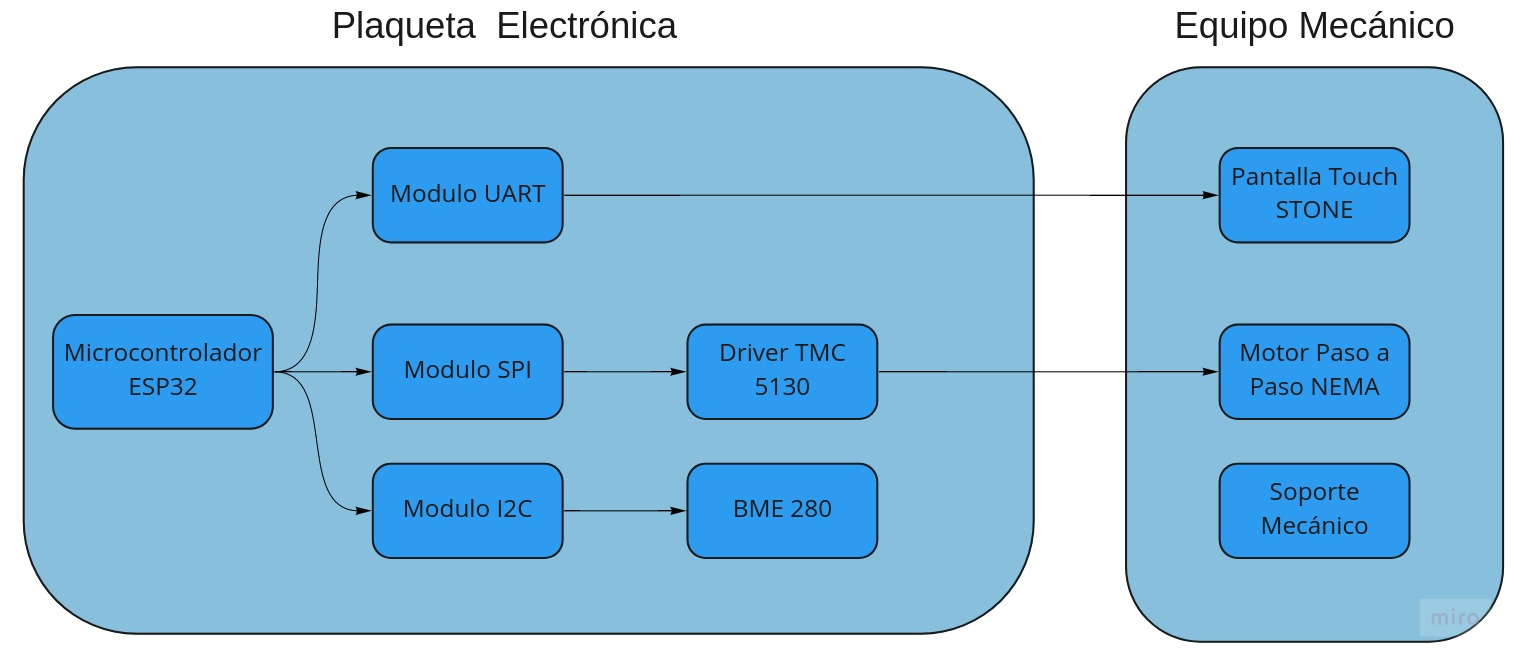
\includegraphics[width=0.9\textwidth]{./Figures/equipo.png}
\caption{Módulos principales de firmware.}
\label{fig:equipo}
\end{figure}
\vspace{25px}


\begin{itemize}
\item Microcontrolador ESP32 
\item Periféricos UART SPI I2C 
\item Driver para manejo de motor TRINAMIC  TMC 5130
\item Comunicación con Stone Display HMI 
\end{itemize}

\section{Movimientos controlados}
\subsection{Integrados Trinamic}
\subsection{Driver TMC5130}

\section{Interfaz de usuario}
\subsection{Pantalla Stone}

\section{Framework de trabajo}

